\section{Auswertung}
\label{sec:Auswertung}

\subsection{Fourier-Synthese}
\noindent Bei der Fourier-Synthese wurde versucht eine 
Sägezahnspannung, eine Rechteckspannung und eine Dreiecksspannung 
darzustelllen. 
\noindent Wenn die Spannungen an den Vielfachen der Grundfrequenz mithilfe des 
Oberwellengenerators so eingestellt werden, ergeben sich die folgenden Fourier-Reihen.
\begin{figure}[H]
    \centering
    \caption{Fourier-Reihe Sägezahnspannung.}
    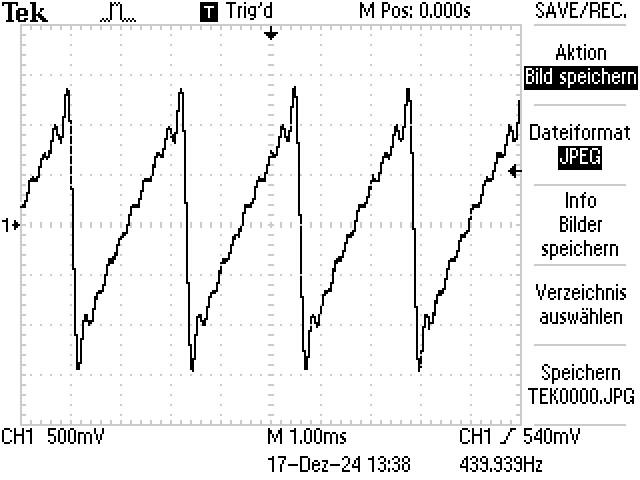
\includegraphics{Bilder/TEK0000.JPG}
\end{figure}

\begin{figure}[H]
    \centering
    \caption{Fourier-Reihe Rechteckspannung.}
    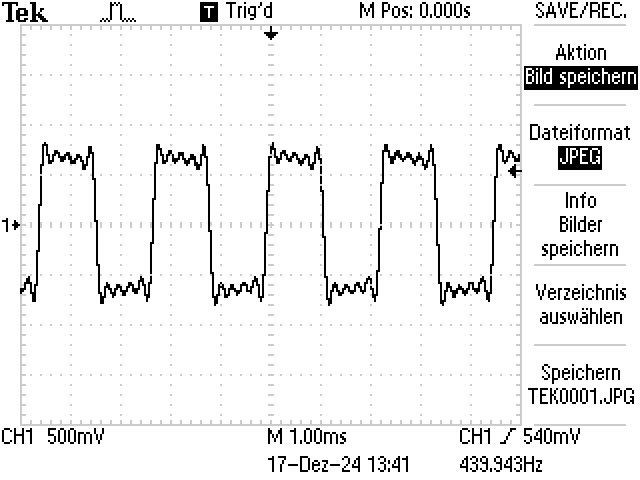
\includegraphics{Bilder/TEK0001.JPG}
\end{figure}

\begin{figure}[H]
    \centering
    \caption{Fourier-Reihe Dreieckspannung.}
    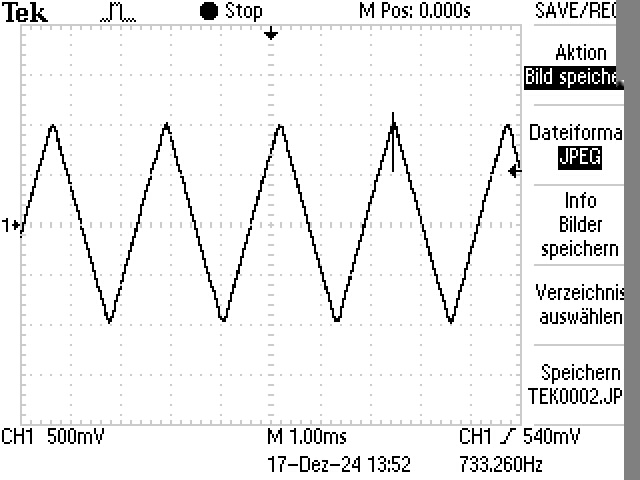
\includegraphics{Bilder/TEK0002.JPG}
\end{figure}


\subsection{Fourier-Analyse}
Bei der Fourier-Analyse werden am Oberwellengeneratur die Rechteckfunktion,
die Dreiecksfunktion und die Sägezahnfunktion generiert. Am Amperemeter werden 
die Amplituden bei den jeweiligen Frequenzen der Oberwelle abgelesen, um so
auf die Abhängigkeit der Spannung der $n$-ten Oberwelle schließen zu können.
\subsubsection{Rechteckspannung}
\begin{table}[H]
    \centering
    \caption{Amplituden der Oberschwingungen Rechteckfunktion.}
    \label{tab:j1}
    \begin{tblr}{
        colspec = {S S S},
        row{1} = {guard, mode=math},
      }
    \toprule
    f (\unit{\hertz}) &  A (\unit{\deci\bel}) & A(\unit{\volt})\\
    \midrule
    10 & 17.8  & 7.76247117\\
    30  & 9.01 & 2.82162958\\
    50  & 4.61 & 1.70019995\\
    70  & 1.81 & 1.23168599\\
    90  &-0.19 & 0.97836295\\
    110 &-1.79 & 0.81376686\\
    130 &-3.39 & 0.67686179\\
    150 &-4.59 & 0.58952198\\
    170 &-6.19 & 0.49034302\\
    190 &-8.19 & 0.38949331\\      
    \bottomrule
    \end{tblr}
\end{table}
\noindent Die Oberwellen sind $n$ Vielfache der Grundfrequenz.
Um auf die Abhängigkeit von $n$ schließen zu können, werden die in Volt 
umgerechnenten Spannungswerte (welche gegen die Ordnung der jeweiligen 
Oberwelle aufgetragen sind) an eine Funktion der Form 
\begin{equation}
    \label{eqn:1}
    U(n) = \frac{a}{n^b}
\end{equation}
\noindent gefittet. Die Umrechnung in Volt wird auf Grundlage der Proportionalität
$\unit{\volt} \propto 10^{\frac{\unit{\decibel}}{20}}$ ausgeführt.

\subsubsection{Rechteckfunktion}
\begin{figure}
    \centering
    \caption{Curve fit und Messwerte der Rechteckspannung.}
    \includegraphics{viereck.pdf}
\end{figure}

\noindent Aus dem Curve fit (erstellt mithilfe der Python Bibiliothek "Pyplot")
ergeben sich für die Rechtecksspannung die Parameter 
\begin{align*}
    a = & \num{7.7 +- 1.0}\\
    b = & \num{1.34 +- 0.26}\\
\end{align*}
\noindent Der Ausgleichsparameter $b$ gibt den Grad der Abhängigkeit von $n$ an.


\subsubsection{Dreieckspannung}
\begin{table}[H]
    \centering
    \caption{Amplituden der Oberschwingungen Dreiecksfunktion.}
    \label{tab:j1}
    \begin{tblr}{
        colspec = {S S S},
        row{1} = {guard, mode=math},
      }
    \toprule
    f (\unit{\hertz}) &  A (\unit{\deci\bel}) & A (\unit{\volt})\\
    \midrule
    10  & 14.2  &5.12861384\\
    30  & -4.59 &0.58952198\\
    50  & -13.4 &0.21379621\\
    70  & -19.4 &0.10715193\\
    90  & -23.4 &0.0676083 \\
    110 & -27.0 &0.04466836\\
    130 & -29.4 &0.03388442\\
    \bottomrule 
    \end{tblr}
\end{table}
\noindent Auch bei der Dreiecksspannung wird ein Curve fit durch eine Funktion
der Form aus \autoref{eqn:1} auf die Messdaten angewendet. 


\subsubsection{Dreiecksfunktion}
\begin{figure}[H]
    \centering
    \caption{Curve Fit und Messwerte Dreiecksspannung}
    \includegraphics{dreieck.pdf}
\end{figure}

\noindent Die Parameter a und b ergeben sich zu 
\begin{align*}
    a = & \num{5.1 +- 1.0}\\
    b = & \num{3.0 +- 2.1}\\
\end{align*}
\noindent Dabei gibt b wieder den Grad der Abhängigkeit an.


\subsubsection{Sägezahnspannung}
\begin{table}[H]
    \centering
    \caption{Amplituden der Oberschwingungen Sägezahnfunktion.}
    \label{tab:j1}
    \begin{tblr}{
        colspec = {S S S},
        row{1} = {guard, mode=math},
      }
    \toprule
    f (\unit{\hertz}) &  A (\unit{\deci\bel}) & A(\unit{\volt})\\
    \midrule
    10  & 11.8  & 3.89045145\\
    20  &  7.01 & 2.24130005\\
    30  &  3.01 & 1.41416473\\
    40  &  1.01 & 1.12331097\\
    50  & -1.39 & 0.85211851\\
    60  & -2.99 & 0.70876131\\
    70  & -4.00 & 0.63095734\\
    80  & -5.79 & 0.51345218\\
    90  & -6.19 & 0.49034302\\
    100 & -8.99 & 0.35522212\\
    110 & -7.79 & 0.40784956\\
    120 & -9.79 & 0.32396642\\
    130 & -9.39 & 0.33923449\\          
    \bottomrule
    \end{tblr}
\end{table}


\subsubsection{Sägezahnfunktion}
\begin{figure}[H]
    \centering
    \caption{Curve fit und Messwerte Sägezahnspannung.}
    \includegraphics{saege.pdf}
\end{figure}
\noindent Die Ausgleichsparameter für die Sägezahnspannung lauten:
\begin{align*}
    a = & \num{4.0 +- 0.9}\\
    b = & \num{0.94 +- 0.28}\\
\end{align*}


%Auskommentiert, da es irgendwie Probleme mit "\includegraphics{rechteck.pdf}"
%gab (bereits bei make nachdem ich direkt gepullt habe)



